\chapter{Metodología}
\section{Introducción}

El Método de Desarrollo de la Arquitectura de TOGAF (ADM) forma el núcleo del TOGAF.  Es un método fiable y de eficacia probada para desarrollar una arquitectura de TI que satisfaga las necesidades comerciales de una organización, utilizando los demás elementos de TOGAF, y otros activos arquitectónicos disponibles para la organización. \\

El TOGAF consta de dos partes principales:

\begin{itemize}
	\item    El Método de Desarrollo de la Arquitectura de TOGAF (ADM).
	\item La Arquitectura de la Fundación TOGAF, la cual se trata de una arquitectura de servicios y funciones genéricas que proporciona una base firme sobre la que se pueden construir arquitecturas y componentes arquitectónicos más específicos.
\end{itemize}

La ADM de la TOGAF describe el proceso de pasar de la Arquitectura de la Fundación TOGAF a una arquitectura específica de la organización (o conjunto de arquitecturas), aprovechando los elementos de la Arquitectura de la Fundación TOGAF y otros componentes arquitectónicos y bloques de construcción pertinentes a lo largo del camino.\\

La Arquitectura de la Fundación TOGAF no es, por supuesto, el único recurso disponible para el arquitecto en el uso de la ADM. Hay una amplia gama de modelos arquitectónicos, componentes y bloques de construcción relacionados con diferentes aspectos del dominio de la arquitectura. Este contexto mucho más amplio en el que reside la Arquitectura de la Fundación TOGAF se denomina en la TOGAF el Continuo Empresarial.\\

Es importante señalar que, al ejecutar la ADM, el arquitecto no sólo está desarrollando el resultado final de una arquitectura específica de la organización, sino que también está poblando el propio Continuo Empresarial de la organización, con todos los activos arquitectónicos identificados y apalancados a lo largo del camino - incluyendo, pero no limitado a, la arquitectura específica de la organización resultante.\\

Aunque el enfoque principal de la ADM está en el desarrollo de la arquitectura específica de la organización, en este contexto más amplio la ADM también puede verse como el proceso de poblar el Continuo Empresarial de la organización con bloques de construcción reutilizables relevantes.\\

El desarrollo de la arquitectura es un proceso iterativo y continuo, y al ejecutar la ADM repetidamente a lo largo del tiempo, el arquitecto va poblando gradualmente más y más el Continuo Empresarial de la organización.\\

De hecho, la primera ejecución del ADM será a menudo la más difícil, ya que los activos arquitectónicos disponibles para su reutilización serán relativamente pocos. Sin embargo, las ejecuciones posteriores serán más fáciles, ya que cada vez se identifican más activos de arquitectura, que se utilizan para poblar el Enterprise Continuum de la organización y, por lo tanto, están disponibles para su reutilización.

\newpage
\section{ADM}
\begin{figure}[h!]
	\centering
	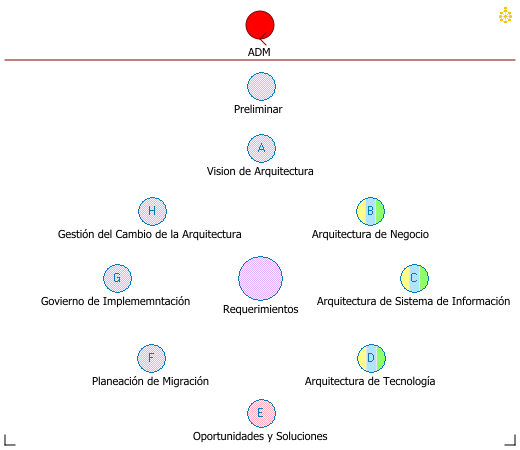
\includegraphics[width=1\linewidth]{imgs/adm.png}
	\caption{ADM \cite{archi3.1,a1,a2,a3,a4}}
\end{figure}
